% DO NOT COMPILE THIS FILE DIRECTLY!
% This is included by the the driver file (FlipBeamerTemplate.tex).

%{ %% This is a total kludge for a fancy title page background
%\setbeamertemplate{sidebar right}
 {\setbeamertemplate{sidebar right}{\llap{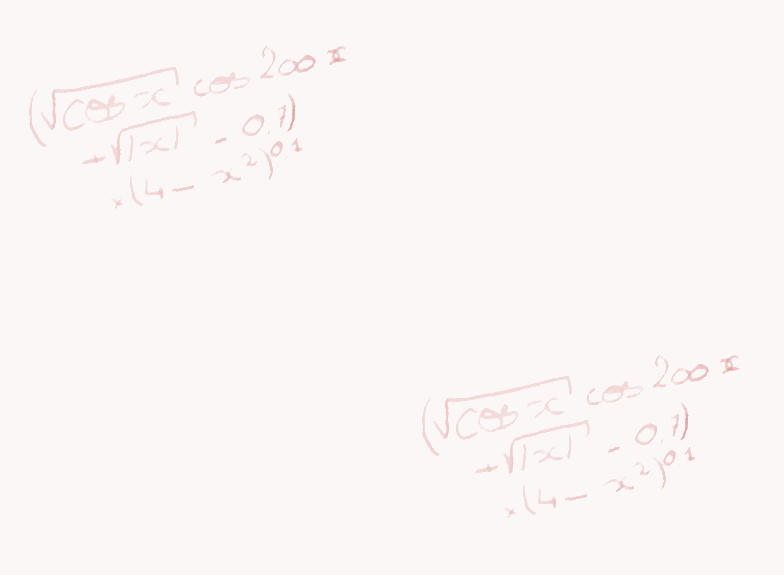
\includegraphics[width=\paperwidth,height=\paperheight]{BG_upper}}}
\begin{frame}[c]%{\phantom{title page}} 
% The \phantom{title page} is a kludge to get the red bar on top
% \titlepage
\begin{center}
	% \includegraphics[width=7cm]{WarpedPenguinsReturn}
%\vspace*{-2cm}
	\begin{tikzpicture}%[show background grid] %% Use grid for positioning, then turn off
		\node[inner sep=10pt,anchor =north west] (title) 
			{ \includegraphics[width=7cm]{\titleimage} };
			 \node (title) at (0.5,-2.5) {};
	\end{tikzpicture}
	\quad

	% \includegraphics[width=7cm]{\titleimage} 
	%\vspace*{1cm}
	\tiny{Céline Caldini-Queiros, Bruno Després, Lise-Marie Imbert-Gérard, Maryna Kachanovska\\ (with Olivier Lafitte and Remi Sart)}
	\vspace{.5em}
	
	\footnotesize\textcolor{brunfonce}{08.04.2014}
%	\texttt{[arXiv:1234.5678]}
	\vspace{1cm}
%	

\end{center}
\end{frame}}
\begin{frame}{Modelisation}
 \begin{minipage}{0.45\linewidth}
 \begin{figure}
       		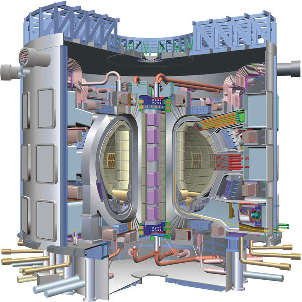
\includegraphics[scale = 0.7]{./images/ITER_cut}
       	\caption{ITER}
     	 \end{figure} 
\end{minipage}
\hfill
\begin{minipage}{0.45\linewidth}
 \begin{figure}
       		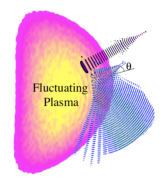
\includegraphics[scale = 1.2]{./images/antenne}
       		\caption{waves}
     	 \end{figure} 
\end{minipage}
\begin{block}{Equations : Maxwell-Newton}
\[
\begin{cases}
&-\frac{1}{c^2}\partial_t E + \nabla \wedge B = \mu_0 J \hspace{3cm} J = e N_e u_e\\
&\partial_t B + \nabla \wedge E  = 0	\\
&m_e \partial_t u_e  =  -e(E + u_e \wedge B_0 ) - m_e \nu u_e
\end{cases}
\]
\end{block}


\end{frame}
\begin{frame}{References}
\begin{itemize}
\item Décomposition de domaines pour la simulation "full wave" dans un plasma froid T. Hattori (thesis) \\ \ \\
\item Analyse mathématique et numérique de problèmes d’ondes apparaissant dans les plasmas
magnétiques, L.-M. Imbert-Gérard (thesis)\\ \ \\
\item Hybrid resonance of Maxwell's equations in slab geometry, B.Després, L.M. Imbert-Gérard and R. Weder, in JMPA\\ \ \\
\item  Stable coupling of the Yee scheme with a linear current model, F. Da Silva, M. Campos-Pinto, B. Després, S. Heuraux, HAL preprint 2014 . \\ 
\end{itemize}
\end{frame}
\begin{frame}{Frequency domain study}
In 1D : $\partial_t = \imath \theta$


\alert{Variational formulation :}
\[
\begin{array}{l}
\displaystyle \int_{-L}^H (E_2' -\imath\theta E_1)\overline{(\tilde E_2' -\imath \theta \tilde E_1)} - \int_{-L}^H (\eps_0 +\imath\nu Id) \E \cdot \overline{\tilde \E}
\\ \displaystyle  - \imath \sqrt{\alpha(-L)} E_2 (-L) \tilde E_2 (-L) = -g_{inc} (-L) \overline{( \tilde E_2(-L) )} 
\end{array}
\]
\[
a(\ubf,\vbf) = a_1 (\ubf,\vbf) +\imath a_2(\ubf,\vbf)\  \text{ and } \  l(\vbf) = -g_{inc} (-L) \overline{(v_2(-L) )} 
\]
\[
\left\{\begin{array}{l}
a_1(\ubf,\vbf) = \int_{-L}^H (u_2' -\imath\theta u_1)\overline{(v_2' -\imath \theta v_1)} - \int_{-L}^H \eps_0 \ubf\cdot \overline{\vbf}, 
\\ a_2(\ubf,\vbf) = -\nu \int_{-L}^H  \ubf\cdot \overline{\vbf} -  \sqrt{\alpha(-L)} u_2 (-L) \overline{v_2 (-L)} , 
\end{array}\right.
\]
where $a_1= a_1^*$ and $a_2=a_2^*$ are hermitian.
\begin{block}{}
\[
|a(u,u)| \geq \min\left(\frac{1}{4} \frac{\sqrt{\alpha(-L)}}{|\Omega|} , \frac{1}{16}\frac{\sqrt{\frac{\nu}{\heps + \theta^2}}}{|\Omega|^2}\right) \|u\|^2_{L^2}
\]
\end{block}
\end{frame}

\begin{frame}{Simulation in frequency domain}
\ALERT{Matlab code, $P^1$ FEM}

 \begin{minipage}{0.7\linewidth}
 \begin{figure}
       		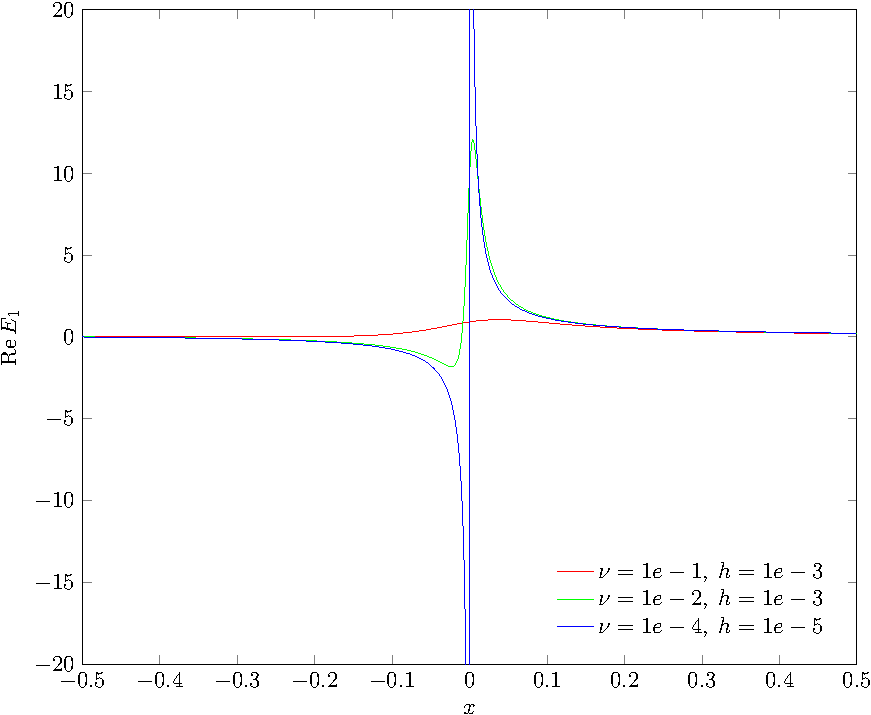
\includegraphics[scale = 0.6]{./images/picture2}
       	\caption{ITER}
     	 \end{figure} 
\end{minipage}
\hfill
\begin{minipage}{0.25\linewidth}
\[
E_\nu \approx \frac{c}{x + \imath \nu}
\]
\end{minipage}
\end{frame}
 {\setbeamertemplate{sidebar right}{\llap{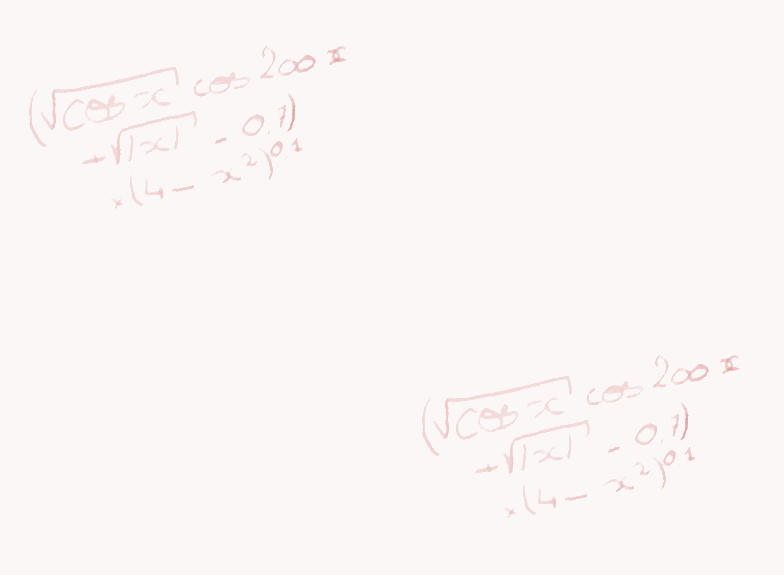
\includegraphics[width=\paperwidth,height=\paperheight]{BG_upper}}}
\begin{frame}
\begin{center}
\textcolor{lightred}{\scalebox{2}{Thank you for your attention !}}
\end{center}
\end{frame}}
